\documentclass[nynorsk,12pt,a4paper]{article}
\usepackage[utf8]{inputenc}
\usepackage{graphicx}
\usepackage{babel}
\renewcommand*{\familydefault}{\rmdefault}
\title{Visjonsdokument\\
Dynamisk Nettverksbrannmur
}
\author{Espen Gjærde \\
Bachelorstudent \\
Avdeling for Informatikk og e-Læring \\
Høgskulen i Sør-Trøndelag \and Svein Ove Undal\\
Bachelorstudent \\
Avdeling for Informatikk og e-Læring \\
Høgskulen i Sør-Trøndelag}
\date{15.02.2013}

\pagenumbering{arabic}
\begin{document}
\maketitle
\newpage

\section*{Revisjonshistorie}

\begin{table}[h!]
	\begin{tabular}{ l l l l }

		\textsc{Dato} & \textsc{Versjon} & \textsc{Beskrivelse} & \textsc{Forfatter} \\
		\hline 
		01.12.2012 & 1.0 & Dokumentet opprettet & Espen, Svein \\ 
		15.02.2013 & 1.0 & Dokument klar for revisjon & Espen, Svein \\ 
		09.04.2013 & 1.2 & Tabellar oppdattert, små rettingar & Espen \\ 
		\hline
	\end{tabular}
\end{table}

\newpage
\tableofcontents{}

\newpage

\section{Innleiing}
\paragraph{}
Dette dokumentet er ei analyse av prosjektet som skal gjennomførast, med mål om å avgjere om prosjektet bør startast. Vi vil i dokumentet gå gjennom bakgrunn og mål for prosjektet, greie ut om interessentar og utføre kost/nytte og risikoanalyse. Vi vil også gå gjennom teknologival, standardar for gjennomføring og suksessfaktorar.

\newpage
\section{Bakgrunn for prosjektet}
\paragraph{}
Prosjektet er ei bacheloroppgåve for Espen Gjærde og Svein Ove Undal. Begge studentar ved Avdeling for Informatikk og e-Læring ved \ Høgskolen i Sør-Trøndelag. Prosjektet går ut på å lage ein smart brannmur basert på pålogging via web. Etter dette skal brukeren få tilpassa reglar for sin bruker. 

\subsection{Skildring av problem og behov}
\paragraph{}
For administratorar av nettverk med mange brukarar -- og mange forskjellige typar brukarar -- kan det være vansklig å halde oversikt over nettilgang \ og effektivt og rettferdig fordle bandbredde og tilgangar mellom brukarene. Spesielt gjeld dette midlertidige nettverk - tildømes dataparty, eller trådløse gjeste-nett. Vi tek sikte på å lage eit system som sikrar rettferdig og dynamisk deling av bandbredde, samstundes som det gir rom for å spesialisere reglar for den enkelte brukar. 

\subsection{Skildring av dagens system og rutiner}
\paragraph{}
Det finnast i dag døme på system der brukarar må logge inn for å nytte seg av ressursar. Dette er gjerne måten adgangskontroll for trådlausnett vert gjort på på flyplassar og hotell. Dette er det som blir kalla captive-portal\footnote{\ Captive{}-Portal: System som tvingar brukarar via ei bestemt nettside eller gjennom eitt spesielt punkt. }. Problemet med slike løysingar er at det enten er fritt fram etter du har logga inn, eller at kapisteten blir delt etter eit <<one-size-fits-all>>-prinsipp. Systema har og svakhetar som mac-addresse spoofing \footnote{forfalsking av unik  adresse eller identifikasjon} og dns-tunnel som ein måte å ungå autentiseringa heilt

\newpage
\section{Prosjektmål}
\paragraph{}
Overordna prosjektmål
\begin{itemize}
	\item lage eit effektivt brannmursytem som er enkelt å nytte seg av
	\item tilegne oss meir erfaring og kompetanse
	\item lage eit solid og stabilt sluttprodukt
\end{itemize}

\paragraph{}
For å beskrive måla med prosjektoppgava er det hensiktsmessig å dele måla inn i føljande kategoriar:
\begin{description}
	\item[Effektmål] --- skildrar effekten sluttbrukar får av å bruke systemet
	\item[Resultatmål] --- skildrar kva som skal ligge føre når prosjektet er ferdig
	\item[Prossessmål] --- mål utviklarane har med å delta i prosessen
\end{description}

\subsection{Effektmål}
\begin{itemize}
	\item Enklere administrajon av brukere i midlertidige nett
	\item Dynamiske brannmurregler og enkel administrering av desse
\end{itemize}

\subsection{Resultatmål}
\begin{itemize}
	\item Eit fullverdig brannmursystem med innlogging
	\item Ein fungerande brannmur med individuelle reglar for kvar brukar eller gruppe
	\item Eit enkelt og oversiktleg administrajonsystem for brannmuren.
	\item Eit system som sjekkar nettverkskonfigurasjon for pålogga maskiner.
	\item Ein pakke med enkel installasjon - gjerne .deb eller tar.gz.
\end{itemize}

\subsection{Prosessmål}
\begin{itemize}
	\item Videreutvikle kunnskapar om linux og nettverksikkerhet
	\item Erfaring med utvikling i python
	\item Utvikling av eit open source distrubuert system
\end{itemize}

\subsection{Prosjektets omfang}
\begin{itemize}
	\item Det skal vere alternativ å lage informasjon som filer, eller i ein database
	\item Det ska implementeres ein oversiktlig administrasjonspanel
	\item Prosjektet skal være ferdigstillit innen 25.mai 0213.
	\item Systemet blir utvikla og testa for Debian 6.0.6 “wheezy”
\end{itemize}

\subsection{Prosjektets milepælar og hovudaktivitetar}

\subsubsection{Dokumentasjon}
\begin{table}[h!]
	\begin{tabular}{ l l } 
		\textsc{Dato} & \textsc{Milepæl} \\ \hline
		04.02.2013 & Oppstart av prosjektet \\ 
		15.02.2013 & Visjonsdokument til revisjon	\\ 
		10.03.2013 & Kravdokument til revisjon	\\ 
		01.04.2013 & Arkitekturdokument til revisjon \\ 
		25.05.2013 & Sluttrapport ferdig og levert	\\ 
		\hline
	\end{tabular}
\end{table}

\subsubsection{Utviklingsteg / Mål}
\begin{table}[h!]
	\begin{tabular}{ l l }
		\textsc{Dato} & \textsc{Milepæl} \\ \hline
		15.02.2013 & Captive-Portal i funksjon \\ 
		20.02.2013 & Brannmur og innlogging styrast av python	\\ 
		08.03.2013 & Prototype klar til test på TIHLDE-LAN \\ 
		20.03.2013 & IPv6 innført i systemet	\\ 
		01.04.2013 & Administrasjonspanel i testversjon \\ 
		01.05.2013 & Release Candidate 1 klar	\\ 
		\hline
	\end{tabular}
\end{table}

\subsection{Teknologi}
\paragraph{}
Vi vil basere prosjektet på eksisterende teknologi og programmer med åpen kjeldekode. Vi vil utvikle systemet i Debian Linux, men systemet skal kunne kjøre på alle linuxplatformer. Mykje av dei programma vi nyttar finnast også til andre *nix-systemer, og burde med enkle steg kunne nyttast her også. Nedanfor vil vi kort grunngi forskjellige val av teknologi. 
\paragraph{Debian Linux Wheezy}
Debian er den Linuxdistibusjonen med åpen kildekode som er sikrast og mest utbreidd. Det gjere Debian som eit lett valg til vårt prosjekt. I tillegg til dette er Debian den linuxversjonen vi har mest erfaring med.
\paragraph{PHP}
For administrasjon og pålogging vil vi nytte webteknologien PHP. Dette er fordi php er et enkelt webspråk som kan kjøres på de fleste platformer og webservere. Det er også et lett språk for en tjener å kjøre.
\paragraph{Python}
Som kodespråk mot systemet nyttar vi oss av python. Slik får vi eit abstraksjonsnivå mellom kode og system, som vi ikkje får med bash-script. Dette gjer det også enklare å portere systemet over til andre platformer enn Debian Linux. 
\paragraph{ISC DHCP-server}
Dette er ein av dei mest utbredte dhcp-tjenarane i marknaden, og er den klart mest brukte i linux-verda. Vi finn det naturlig å nytte denne både fordi kildekoden er åpen, og fordi det gjer eventuell interasjon mellom systemet vi utvikar og eventuelle eksisterande system enklare. 
\paragraph{IPtables}
For sjølve brannmuren vil vi nytte iptables. Dette er en enkel pakkefiltrerande brannmur som er støtta i dei fleste *nix-systemer. 
\paragraph{Brukerdatabase - PAM} 
Vi vil kjøre autentisering gjennom Linux PAM\footnote{\ Pluggable Authentiction Modules: Eit fleksibelt authentiseringsystem. Gir mulighet for mange forskjellige typar brukardatabasar.}. Dette gjer at sluttbrukar står fritt til å velje brukerdatabase. For demonstrasjon og testing vil vi bruke OpenLDAP og FreeRadius som brukardatabasar.

\newpage
\section{Interessenter og rammebetingelser}
\subsection{Interessentanalyse}
\begin{table}[h!]
	\begin{tabular}{p{5cm} p{5cm} p{5cm} }
		\textsc{Interessent} & \textsc{Suksesskriterie} & \textsc{Bidrag til prosjektet}\\ \hline \\
		\textbf{Eksterne interessenter} & ~ & ~ \\ 
		Høgskolen i Sør-Trøndelag & Dokumentasjon og kode levert innan frist & Oppdaragsgiver \\ 
		TIHLDE & Programvare stabil under testing & Tilgang til å teste programmet under TIHLDE sitt dataparty. \\ \\
		\textbf{Interne interessenter} & ~ & ~ \\ 
		Studentane & Strukturert jobbing & Systemutviklarar og prosjekteigarar \\ 
		Veileder & God kommunikasjon, hyppig oppdatering & Kunnskap, Veiledning \\ 
	\end{tabular}
\end{table}


\subsection{Rammebetingelser}
\begin{itemize}
	\item Produkt og dokumentasjon ferdig innan 25.mai 2013
	\item Produktet skal kunne installerast og brukast av ein brukar utan store krav til linux/nettverks kunnskap.
	\item Systemet er utvikla og testa i Debian 6.0.6 “Wheezy”
	\item Utviklingsmetoden Unified Process vert nytta.
	\item Systemet vert basert på og utgitt som åpen kildekode. 
\end{itemize}

\newpage
\section{Kritiske suksessfaktorer}
\subsection{Suksessfaktorer}
\paragraph{}
Sømløst system, som fungerer uten at sluttbrukar merker at systemet er der. Systemet skal effektivt gjere nettverket bedre å bruke med tanke på ping og ytelse under stress. 
\paragraph{}
Systemet skal vere særdeles lett å settast opp, det skal ikkje krevast store kunnskapar innan linux og nettverksadministrasjon for å få systemet til å fungere.

\subsection{Informasjonsbehov}
\paragraph{}
Veileder skal haldast oppdatert om framgangen i prosjektet

\newpage
\section{Risikoanalyse}
\begin{description}
	\item[A] Langvarig sjukdom/fravær av gruppemedlemmar
	\item[B] Samarbeidsvanskar i teamet
	\item[C] Feil på programvare vi er avhengig av
	\item[D] Produkt ikkje i kjørbar versjon ved testtid
	\item[E] Programvare oppfører seg ikkje som forutsett
	\item[F] Vanskeleg brukargrensesnitt
	\item[G] For høge systemkrav
	\item[H] Tap av viktig data
\end{description}
\paragraph{}
Sjå Vedlegg A for risikoscore og utreking av sannsyn og konsekvens

\begin{figure}[h!]
	\centering
	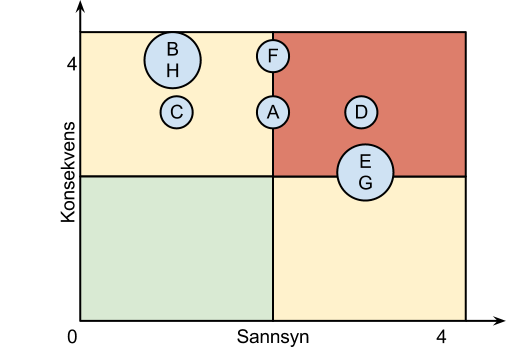
\includegraphics[scale=0.75]{./vdok-img/vdok-ros.png}
	\caption{Identifiserte risikoar plassert i koordinatsystem.}
\end{figure}

\newpage
\section{Kost/nytte-analyse}
\paragraph{}
Dette er eit bachelorprosjekt som baserar seg på bruk av åpen kildekode og alle nytta verktøy er åpne og fritt tilgjengeleg. Vi vil også publisere all kildekode under ein fri lisens. Det er derfor vanskleg å sette opp gode kostnadsvurderingar; arbeidskraft, materia og verktøy er gratis. 

\subsubsection{Kvantifiserbar nytte}
\begin{itemize}
	\item Mindre adminsitrasjonsarbeid for nettverksansvarlig
\end{itemize}

\subsubsection{Ikkje-kvantifiserbar nytte}
\begin{itemize}
	\item Betre fordeling av bandbredde
\end{itemize}

\subsection{Bortfall av direkte kostnadar}

\subsection{Estimerte kostnadar}
\begin{itemize}
	\item Prosjektgruppa består av to studentar som kvar skal arbeide omlag 450 timar
	\item Veiledar har 30 timar til disposisjon for vegleiing
	\item Drift og vedlikehold blir små eller uvensentlige kostnadar. Med tanke på maskinvarekrav skal dette systemet ha svært lave krav. Einaste maskinvare krav er to nettverksportar. 
\end{itemize}

\subsection{Samanstilling av kostnadar og nytte}
\paragraph{}
Det har i dette prosjektet vore vansklig å lage ei klar vurdering av kost og nytte. Vi har få klare kvantifiserbare nytteeffektar, og einaste klare kostnaden timestallet som skal brukast. Dette timetallet er igjen ikkje spesielt for prosjektet, men ein del av eikvar bacheloroppgåve. 

\newpage
\section{Retningslinjer og standardar}
\subsection{Krav til dokumentasjon}
\paragraph{}
Følgande dokumentasjon skal følge
\begin{itemize}
	\item Visjonsdokument
	\item Kravdokument
	\item Arkitekturdokument
	\item Brukerdokumentasjon
	\item Installasjonsvegleiing
	\item Sluttrapport
\end{itemize}

\subsection{Krav til kvalitetskontroll}
\paragraph{}
Kvalitets gjennomgang blir tildels dekket av de daglige utviklingsmøtene i prosjektgruppa. Vi får her tilbakemelding om eventuelle endringer som burde vært endret i systemet, og om det må tilføyes noe. 

\paragraph{}
Prosjektgruppa må også ha en gjennom gang av følgende:
\begin{itemize}
	\item Pythonkode
	\item PHP/HTML-kode
	\item Brukervennlighet på web siden
	\item Databasestruktur og sikkerhet
\end{itemize}

\paragraph{}
I tillegg til å kvalitetssikre, tester vi programvaren underveis og etter kvar endring. Testingen underveis blir en peikepinne på om systemet fungerer som det skal, samt at vi utbedrer alle problemer når de oppstår. Vi vil òg ha ei utbredt testing av ein prototype på TIHLDE{}-lan, som vil effektivt vise svakheter og styrker i systemet.

\subsection{Krav til standardar og metoder}
\paragraph{}
Systemet skal bruke kjent teknologi og basere seg på innførte standardar. Dette fordi det for sluttbrukar sine klientar ikkje skal være behov for spesialutstyr eller eigne klientprogram. 

\subsubsection{Programmeringstandardar}
\begin{itemize}
	\item Programmering skjer i språka HTML, PHP og python.
	\item Alle metodar skal ha engelske navn, og følge kjente namnekonvensjonar i sine respektive språk.
	\item Kommentarar og forklaringar i kodefilene skal skrivast på engelsk.
\end{itemize}

\subsubsection{Konfigurasjonsfiler}
\begin{itemize}
	\item Konfigurasjonsfiler og programvare skal i størst mulig grad følge standardar og ligge der det er naturlig i eit linux / Debian{}-system.
	\item Kommentarar og forklaringar i filene skal skrivast på engelsk
\end{itemize}

\subsubsection{Bruk av verktøy}
\begin{itemize}
	\item Versjonskontroll skjer med versjonshandteringssystemet GIT. 
	\item Systemet blir testa på ei tjenermaskin med operativsystemet Debian 6.0.6 “Wheezy”. 
\end{itemize}
\subsubsection{Andre standardar}
\begin{itemize}
	\item Systemet skal baserast på kjente og de{}-facto standard protokollane IP, TCP, DHCP og HTTP.
	\item Språk for administrajonsystemet skal være norsk - nynorsk.
\end{itemize}

\subsection{Endringshandtering}
\begin{enumerate}
	\item Eventuell mistanke om problemer meldast tidleg til dei andre i prosjektgruppa
	\item Det skal arbeidast med å få oversikt over endringar og ringverknadar.
	\item Endringer dokumenterast og avvik rapporterast
	\item Tidsplaner justerast
	\item Endringer gjennomførast
	\item Evaluering av endring og endringsprosessen vert gjennomført
\end{enumerate}

\newpage
\section{Prosjektorganisering}
\paragraph{}
Prosjektoranisasjonen består av ei prosjektgruppe, studentane, og veileder som også utgjer styringsgruppa.

\begin{figure}[h!]
	\centering
	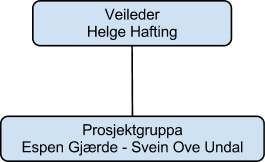
\includegraphics[scale=0.75]{./vdok-img/vdok-org.png}
	\caption{Prosjektorganisasjonen}
\end{figure}

\newpage
\section{Tilråding om vidare arbeid}
\paragraph{}
Med bakgrunn i forstudiearbeidet og dette visjonsdokumentet vert det tilrådd at prosjektet vert utvikla vidare. 

\newpage
\section{Vedlegg}
\begin{table}[h!]
	\begin{tabular}{l l}
		\textsc{Vedlegg} & \textsc{Namn på dokument} \\
		\hline 
		Vedlegg A & Risikoanalyse\\
	\end{tabular}
\end{table}

\end{document}











